\documentclass[12pt, xcolor={dvipsnames}, aspectratio = 169, sans,mathserif]{beamer}

\usepackage{fontspec}
\usepackage{fontawesome5}
\usepackage{mathrsfs}
\usepackage{amsmath, amssymb}
\usepackage{graphicx}
\usepackage{hyperref}
%\usepackage{physics}
\usepackage[absolute,overlay]{textpos}
\usepackage[font=tiny]{caption}
\usepackage[backend=bibtex, style=science]{biblatex}
\usepackage{standalone}
\usepackage{tikz}
\usepackage{braket}
\usetikzlibrary{shapes,arrows}

% Bib file
\addbibresource{MLRefs.bib}


% Custom Beamer theme
% \usetheme{Bergen}

% Define the custom theme
\mode<presentation>


% Modify color scheme
\definecolor{nmsured}{RGB}{137,18,22} % NMSU colors
% \usecolortheme[named=nmsured]{structure}
\setbeamercolor{structure}{fg=nmsured} % Adjust structure color
\setbeamercolor{item}{fg=nmsured}
\setbeamercolor{frametitle}{bg=white, fg=nmsured}
\setbeamercolor{sidebar}{bg=nmsured}

\usefonttheme{serif}
%\setmainfont{Hack}
\setbeamertemplate{footline}[frame number]
\setbeamertemplate{caption}[numbered]
\setbeamerfont{footnote}{size=\tiny}
% Adjust the width of the sidebar
\setbeamersize{sidebar width left=0.5cm}


% Some custom commands
\newenvironment{List}[2]
{\begin{textblock}{#1}#2
\begin{itemize}}
{\end{itemize}
\end{textblock}}

\newenvironment{Pic}[2]
{\begin{textblock}{#1}#2
\begin{figure}}
{\end{figure}
\end{textblock}}

\newcommand{\BeamerCite}[1]{{\tiny \footfullcite{#1}}}

% Title of the slides
\title{Extracting the $\cos2\phi$ Asymmetry in the Drell-Yan process using Deep Neural Networks}
% \subtitle{Subtitle}
\author{Dinupa Nawarathne}
\institute{New Mexico State University \\
  Representing the E906/SeaQuest Collaboration
}

\date{NPML2023 - August 24, 2023}

\titlegraphic{

\includegraphics[height=0.8cm]{imgs/Fermilab_logo.svg.png}

\includegraphics[height=0.8cm]{imgs/NMSU_logo.jpg}

\includegraphics[height=0.8cm]{imgs/SeaQuest.jpg}

\includegraphics[height=0.8cm]{imgs/DOE.png}
}


\begin{document}

\begin{frame}
    \maketitle
\end{frame}

\begin{frame}
    \frametitle{Table of Contents}
    \tableofcontents
\end{frame}

\section{Motivation}
\subsection{Structure of the Proton}

\begin{frame}
\frametitle{Structure of the Proton}

\begin{Pic}{6.0}{(1.0, 2.0)}
    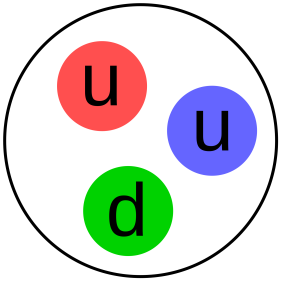
\includegraphics[width=6.0cm]{imgs/proton3.png}
    \caption{Three valance quarks in proton.}
\end{Pic}

\begin{List}{8.}{(7., 4.)}

    \item Protons;

    \begin{itemize}

        \item Spin 1/2 fermions

        \item Composed of three valance quarks: two up ($u$) quarks and one down ($d$) quark

        \item Quarks are bound together by gluons

        \item Properties: mass, charge, \textcolor{red}{spin} etc. $\rightarrow$ 3 valance quarks ?

    \end{itemize}

\end{List}

\end{frame}

\begin{frame}
\frametitle{Structure of the Proton}

\begin{Pic}{7.0}{(1.0, 2.0)}
    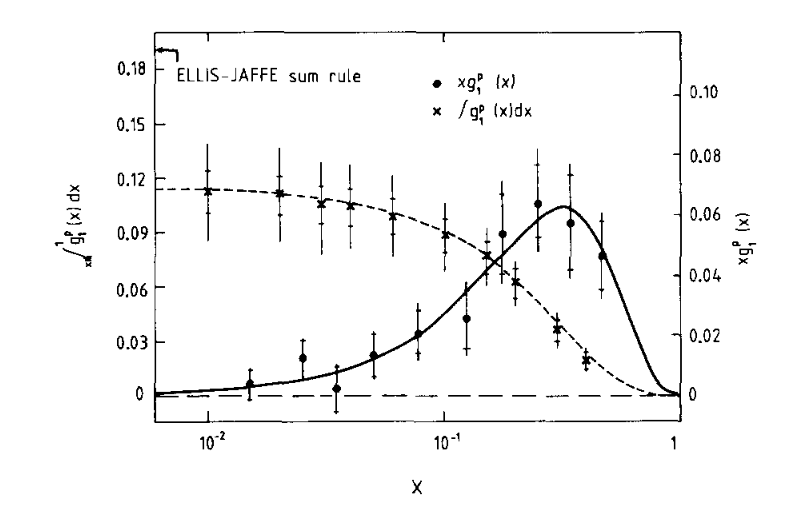
\includegraphics[width=7.0cm]{imgs/EMC.png}
    \caption{EMC result for the proton spin.\BeamerCite{EuropeanMuon:1987isl}}
\end{Pic}

\begin{List}{8.}{(7., 2.)}

    \item European Muon Collaboration (EMC):

    \begin{itemize}

        \item $\text{1}^{\text{st}}$ measurement of the total spin of the proton $\rightarrow$ ``Spin Crisis"

        \item Quarks contributes only $14 \pm 9 \pm 21 \%$ of the proton spin

        \item What contributes to the proton spin ?

    \end{itemize}

\end{List}

\end{frame}


\begin{frame}
\frametitle{Structure of the Proton}

\begin{Pic}{6.}{(1., 2.)}
    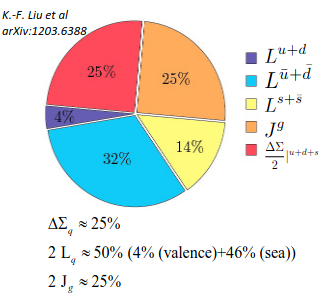
\includegraphics[width=6.0cm]{imgs/spin_decomp.png}
    \caption{Spin Decomposition according to lattice QCD.\BeamerCite{Liu:2021lke}}
\end{Pic}

\begin{textblock}{8.}(8., 2.)
\begin{equation*}
\frac{1}{2} = \frac{1}{2} \Delta \Sigma + \Delta G + L_{q} + L_{\bar{q}} + L_{G}
\end{equation*}

$\frac{1}{2}\Delta \Sigma$ - contribution of the intrinsic spin of the quarks and anti-quarks \\
$\Delta G$ - contribution of the intrinsic spin of the gluons \\
$L_{q}, L_{\bar{q}}, L_{G}$ - contributions of the orbital angular momentum of the valence quarks, sea quarks, and gluons, respectively

\end{textblock}

\end{frame}

\begin{frame}
\frametitle{Structure of the Proton}

\begin{Pic}{6.}{(1., 2.)}
    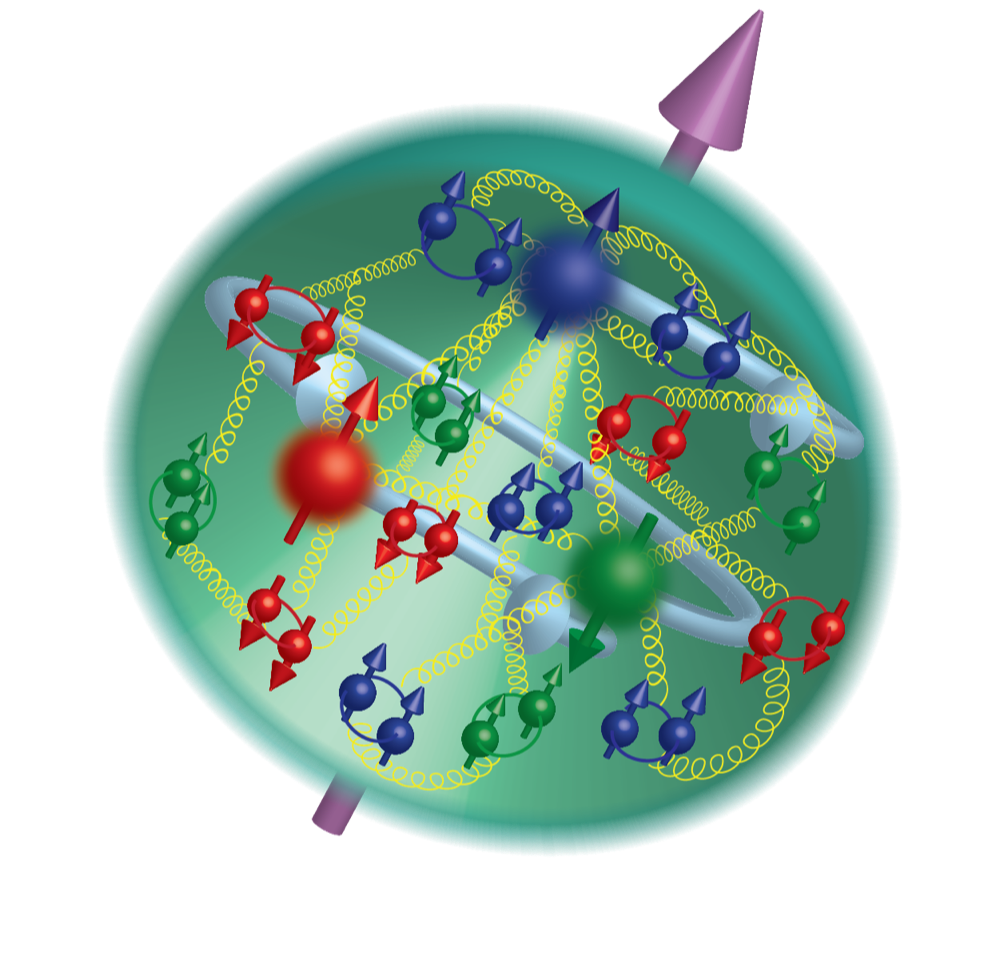
\includegraphics[width=6.0cm]{imgs/dynamic_proton.png}
    \caption{Dynamic structure of the proton.}
\end{Pic}

\begin{Pic}{6.}{(8., 1.)}
    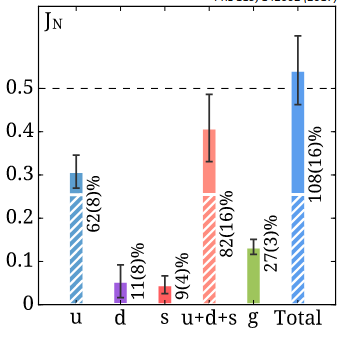
\includegraphics[width=6.0cm]{imgs/J_vbar_211.png}
    \caption{proton spin decomposition in terms of the angular momentum.\BeamerCite{Liu:2021lke}}
\end{Pic}

\end{frame}

\begin{frame}
\frametitle{Structure of the Proton}

\begin{Pic}{6.}{(9., 1.)}
    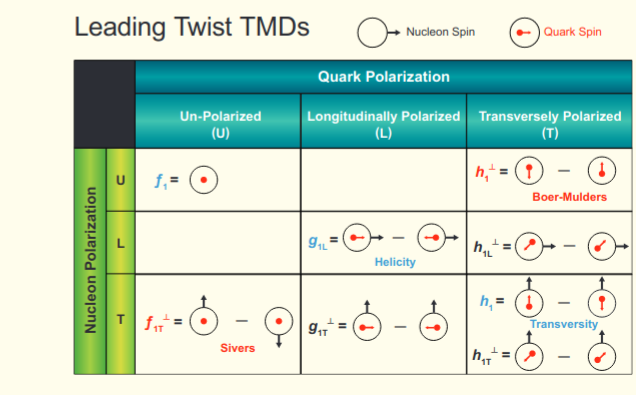
\includegraphics[width=6.0cm]{imgs/TMD.png}
    \caption{TMDs classification according to the polarization of the quarks and nucleon.\BeamerCite{Accardi:2012qut} }
\end{Pic}

\begin{List}{8.}{(1., 2.)}

    \item Transverse momentum distributions (TMDs): distributions of the hadron's quark or gluon momenta that are perpendicular to the momentum transfer between the beam and the hadron

\end{List}


\begin{List}{14.}{(1., 10.)}

    \item Provide information on the confined motion of quarks and gluons inside the hadron and complement the information on the hadron structure.

    \item Boer-Mulders (BM) function: transverse-polarization asymmetry of quarks within an unpolarized hadron

\end{List}

\end{frame}

\subsection{Drell-Yan Process}

\begin{frame}
\frametitle{Drell-Yan Process}

\begin{Pic}{6.}{(8., 2.5)}
    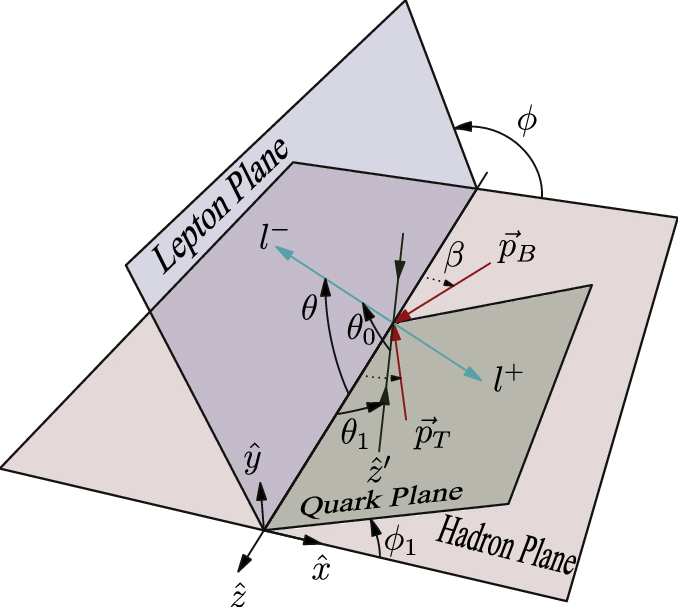
\includegraphics[width=6.0cm]{imgs/three_plane_newest.png}
    \caption{Diagram of the Collins-Soper frame.\BeamerCite{Peng:2018tty}}
\end{Pic}

\begin{Pic}{6.}{(1., 2.)}
    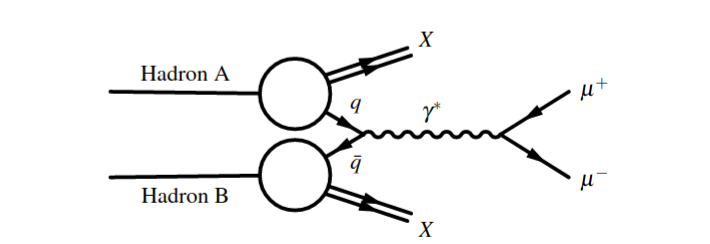
\includegraphics[width=6.0cm]{imgs/drell-yan.png}
    \caption{Drell-Yan process.\BeamerCite{Nagai:2017fcp}}
\end{Pic}


\begin{textblock}{8.}(7., 1.)
\begin{equation*}
\frac{d\sigma}{d\Omega} \propto 1  + \lambda \cos^{2}\theta + \mu \sin 2 \theta \cos \phi + \frac{1}{2}\nu \sin^{2}\theta \cos 2 \phi
\end{equation*}
\end{textblock}

\begin{List}{8.}{(1., 8.5)}

    \item Drell-Yan process $\rightarrow$ probing the internal structure of hadrons

    \item Extraction of $\nu$ parameter $\rightarrow$ BM function

\end{List}

\end{frame}

\begin{frame}
\frametitle{Boer-Mulders Function ($h_{1}^{\perp}$)}

\begin{Pic}{6.}{(1., 3.)}
    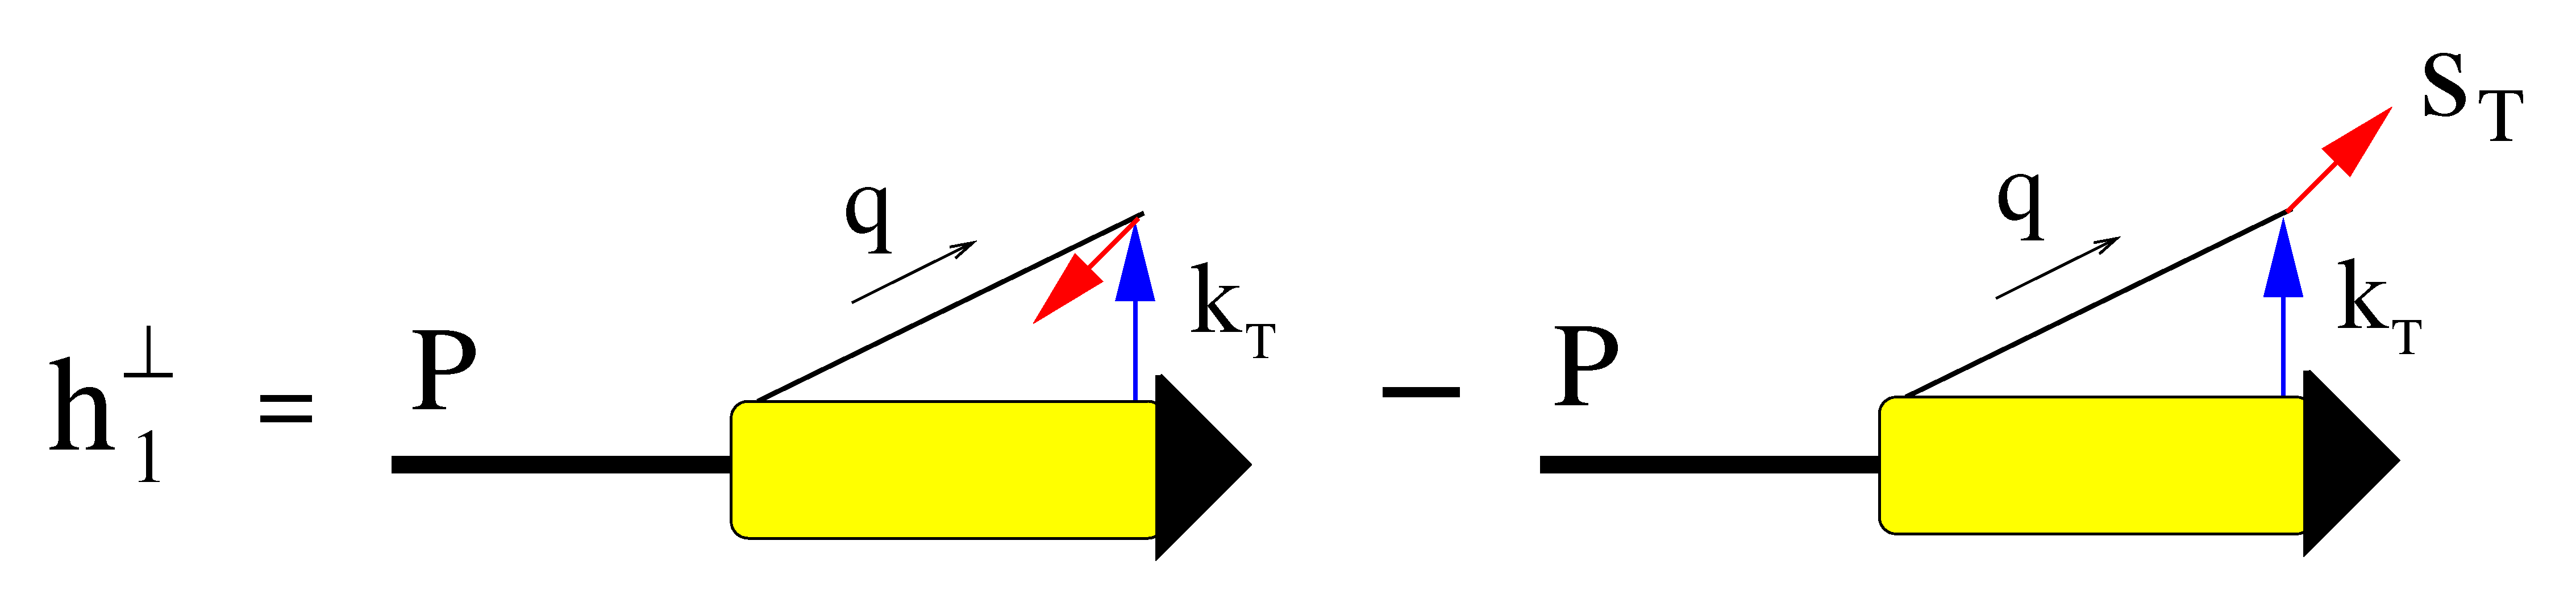
\includegraphics[width=6.0cm]{imgs/BMF.png}
    %\caption{Parameter $\nu$ vs. $p_{T}$ for Drell-Yan process in E866 experiment.\BeamerCite{NuSea:2006gvb}}
\end{Pic}

\begin{textblock}{8.}(5., 1.5)
\begin{equation*}
h_{1}^{\perp [C]} (x, k_{T}^{2})\epsilon_{T}^{ij}k_{T_{j}} = \frac{M}{2} F.T. \braket{P|\bar{\psi}(0)\mathcal{L}_{c}(0, \varepsilon)\gamma^{i}\gamma^{\dagger}\gamma_{5}\psi(\varepsilon)|P}
\end{equation*}
\end{textblock}

\begin{List}{8.}{(7., 4.5)}

    \item  Describes the net polarization of quarks inside an unpolarized proton

\end{List}

\begin{List}{14.}{(1., 7.)}

    \item Quarks can be polarized on average even inside an unpolarized proton, as long as they are not moving exactly along the proton direction.

    \item If $h_{1}^{\perp} \neq 0$ $\rightarrow$  then it reflects the presence of a handedness inside the proton $P\cdot(k_{T} \times s_{T})$

    \item $h_{1}^{\perp}$ $\rightarrow$ quark distribution that quantifies a particular spin-orbit correlation

\end{List}

\end{frame}

\begin{frame}
\frametitle{Evidence for Non-zero BM Function}

\begin{Pic}{6.}{(1., 1.5)}
    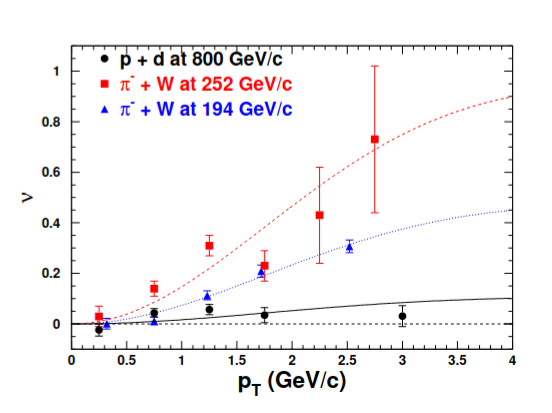
\includegraphics[width=6.0cm]{imgs/nu_E866.png}
    \caption{Parameter $\nu$ vs. $p_{T}$ for Drell-Yan process in E866 experiment.\BeamerCite{NuSea:2006gvb}}
\end{Pic}

% \begin{List}{8.}{(1., 12.)}
%
%     \item Evidence for polarized quark in unpolarized proton.
%
% \end{List}

\begin{Pic}{9.}{(7., 1.5)}
    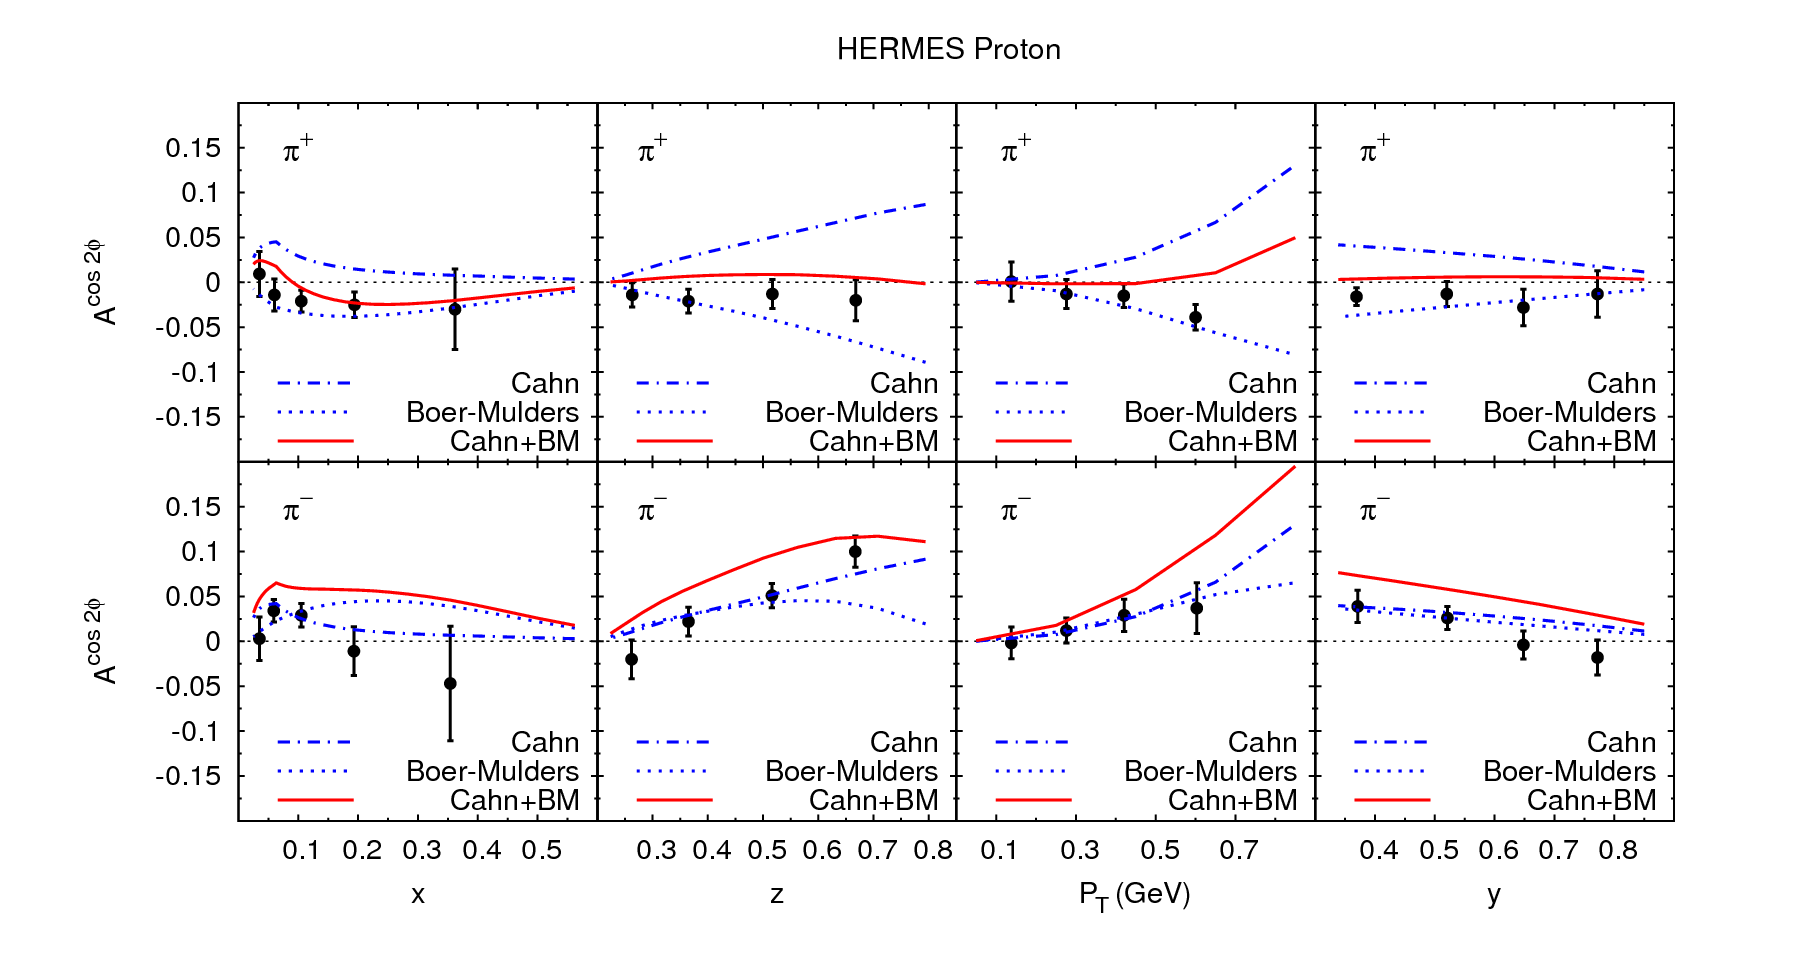
\includegraphics[width=9.0cm]{imgs/BM.png}
    \caption{HERMES proton-target data for SIDIS process.\BeamerCite{Barone:2009hw}}
\end{Pic}

\end{frame}

\section{SeaQuest/E906 Experiment}

\begin{frame}
\frametitle{SeaQuest/E906 Experiment}

\begin{List}{7.}{(1., 2.)}

    \item Fixed target Drell-Yan experiment at Fermilab

    \item Use 120GeV beam energy from the main injector

    \item Measure the antiquark structure of the nucleon

    \item Provides unique access to the vanishing sea quark density at high $x$

    \item Data collection was concluded in 2017

\end{List}

\begin{Pic}{7.}{(8., 2.)}
    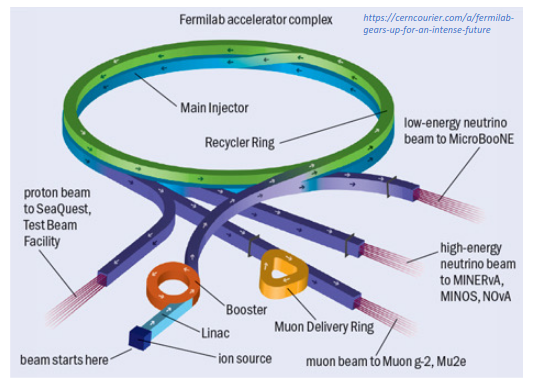
\includegraphics[width=7.cm]{imgs/injector.png}
    %\caption{SeaQuest/E906 spectrometer.\BeamerCite{SeaQuest:2017kjt}}
\end{Pic}

\end{frame}

\begin{frame}
\frametitle{SeaQuest/E906 Experiment}

\begin{Pic}{12.}{(1., 1.)}
    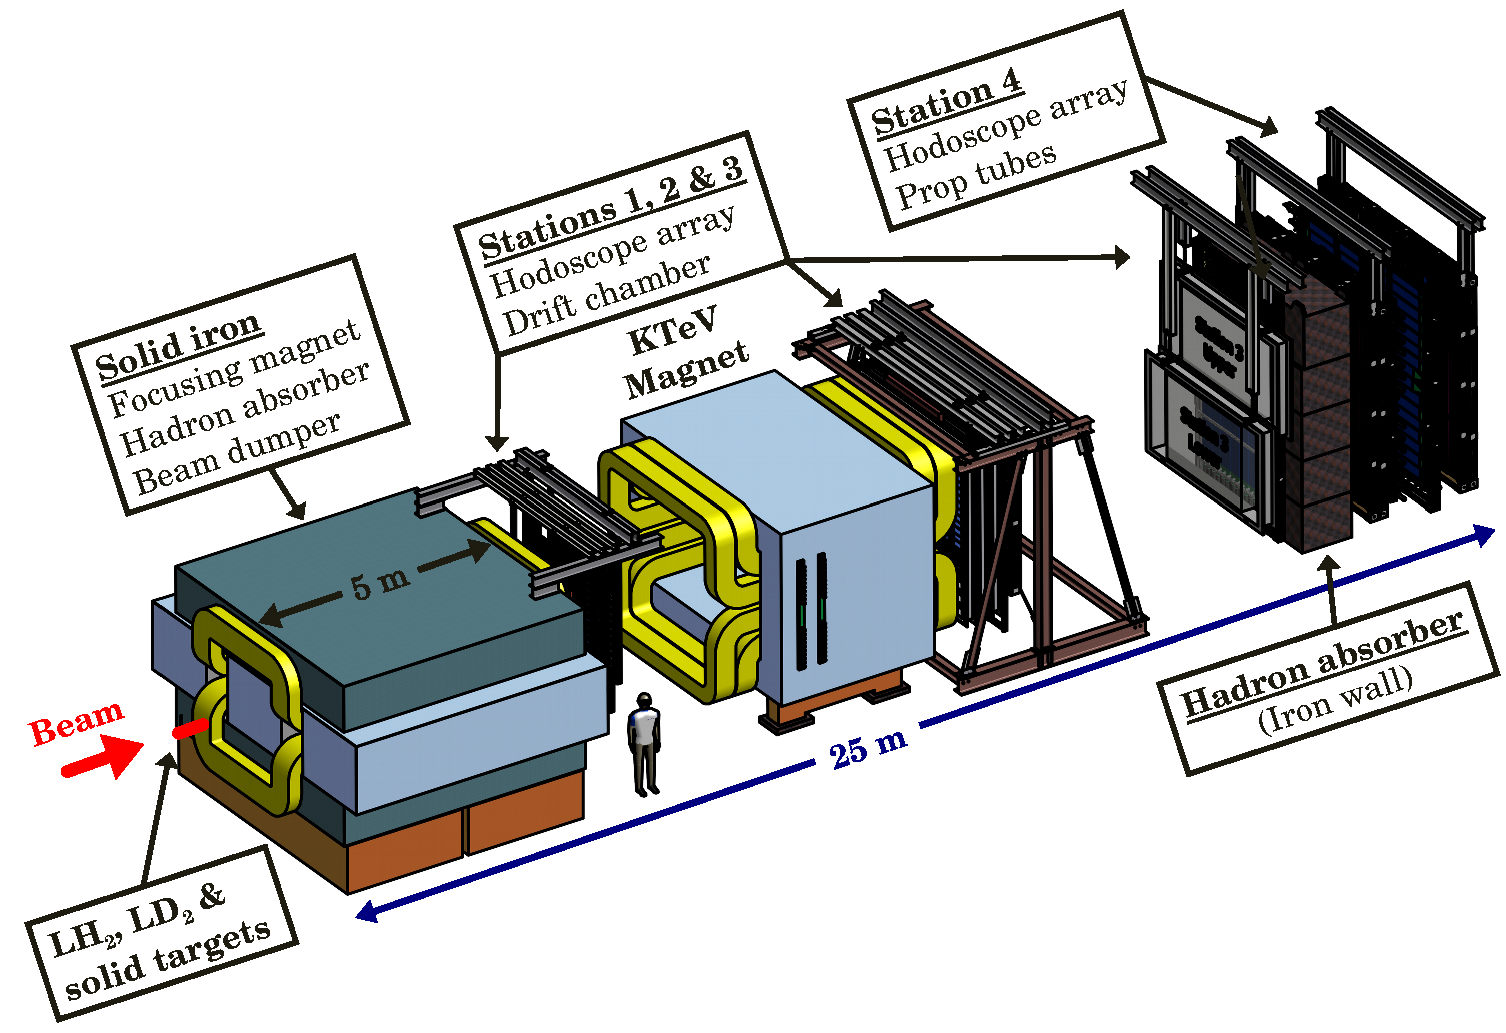
\includegraphics[width=11.cm]{imgs/spectrometer.pdf}
    \caption{SeaQuest/E906 spectrometer.\BeamerCite{SeaQuest:2017kjt}}
\end{Pic}

\end{frame}

\begin{frame}
\frametitle{SeaQuest/E906 Experiment}

\begin{Pic}{8.}{(1., 2.)}
    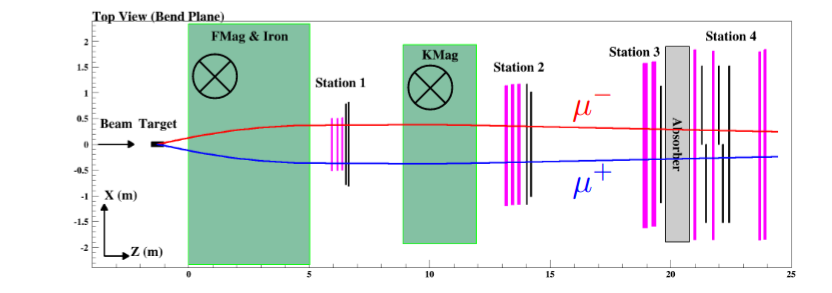
\includegraphics[width=8.cm]{imgs/mup_mum.png}
    \caption{Top view of the detector and muon pair track.\BeamerCite{Nagai:2017fcp}}
\end{Pic}

\begin{Pic}{6.}{(9., 2.)}
    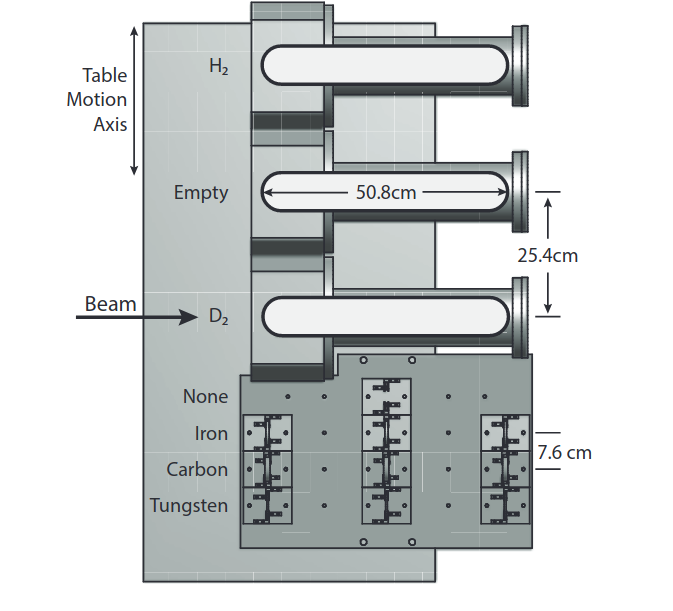
\includegraphics[width=6.cm]{imgs/target.png}
    \caption{Targets used in the SeaQuest experiment.}
\end{Pic}

\begin{Pic}{7.}{(1., 9.)}
    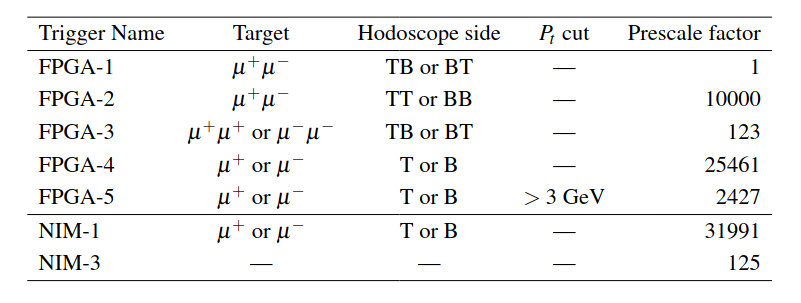
\includegraphics[width=7.cm]{imgs/trigger.png}
    %\caption{Targets used in the SeaQuest experiment.}
\end{Pic}

\end{frame}

\section{Deep Neural Networks for Extracting the $\cos 2 \phi$ Asymmetry in the Drell-Yan process}
\subsection{Likelihood Ratio fit Method with Deep Neural Networks}

\begin{frame}
\frametitle{Analysis Procedure}

\begin{List}{14.}{(1., 2.0)}

  \item Experimental data $\rightarrow$ need corrections for detector acceptance, inefficiencies, smearing etc.

  \item Traditional ``Unfolding'': map detector level information $\rightarrow$ particle level

  \begin{itemize}
    \item Usually, this is done through matrix manipulations

    \item Does not scale well in higher-dimensional parameter space
  \end{itemize}

  \item Deep neural networks (DNN) $\rightarrow$ excellent non-linear functional approximators;

  \begin{itemize}
    \item Parameterize DNN classifiers $\rightarrow$ the Drell-Yan angular coefficients at the particle level

    \item Likelihood ratio test $\rightarrow$ extract the Drell-Yan angular coefficients
  \end{itemize}

  \item DNN approach $\rightarrow$ higher-dimensional phase space $\rightarrow$ directly extract the Drell-Yan coefficients at the particle level

\end{List}
\end{frame}

\begin{frame}
\frametitle{Likelihood Ratio Test}

\begin{List}{14.}{(1., 2.)}

    \item The likelihood ratio test is a highly effective method for assessing the goodness of fit.

    \item Let $X_1, X_2, X_3, \ldots, X_n$ be a random sample from a distribution with a parameter $\theta$. Suppose that we have observed $X_1 = x_1, X_2 = x_2, \ldots, X_n = x_n$. We define the the likelihood function as the joint probability of the observed samples as a function of $\theta$;

    \begin{equation*}
    \mathcal{L}(x_1, x_2, \ldots, x_n; \theta) = P(X_1=x_1, X_2=x_2, \ldots, X_n=x_n; \theta)
    \end{equation*}

    \item To decide between two simple hypotheses $H_0: \theta = \theta_0$ and $H_1: \theta = \theta_1$, we define the likelihood ratio:

    \begin{equation*}
    \lambda(x_1, x_2, \ldots, x_n) = \frac{\mathcal{L}(x_1, x_2, \ldots, x_n; \theta_0)}{\mathcal{L}(x_1, x_2, \ldots, x_n;\theta_1)}
    \end{equation*}

\end{List}

\end{frame}


\begin{frame}
\frametitle{Likelihood Ratio Test}

\begin{List}{14.}{(1., 2.)}
    \item To perform a likelihood ratio test, we choose a constant $c$. We reject $H_0$ if $\lambda < c$ and accept it if $\lambda \geq c$. The value of $c$ can be chosen based on the desired significance level $\alpha$.

    \item Neural networks excel at approximating non-linear functions, making them ideal for use as higher dimensional likelihood functions.

    \item Our goal is to train the neural network to classify samples accurately. Specifically, we aim to classify samples $\omega_{0i} \in \Omega_0$ as $y = 0$ and $\omega_{1i} \in \Omega_1$ as $y = 1$, regardless of the parameter $\theta$.

    \item Subsequently, we can utilize the trained neural network to estimate any unknown parameter $\theta_{\text{unknown}}$ by employing the gradient descent algorithm.\BeamerCite{Andreassen:2019nnm}

\end{List}

\end{frame}

\begin{frame}
\frametitle{Likelihood Ratio Test}

\begin{Pic}{6.0}{(1., 2.)}
\scalebox{0.7}{
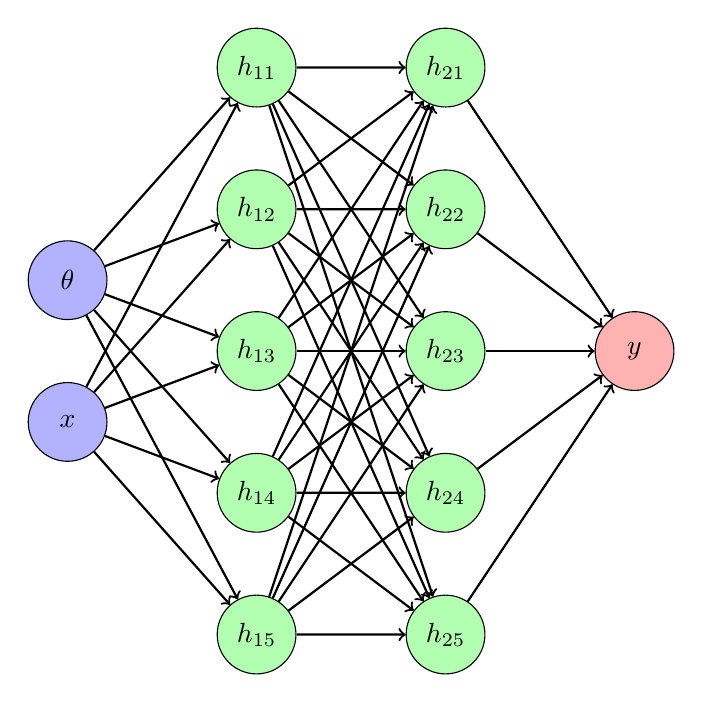
\begin{tikzpicture}[scale=1.2, every node/.style={draw, circle, minimum size=1cm}]
  % Input Layer
  \node[fill=blue!30] (input1) at (0,0.75) {$\theta$};
  \node[fill=blue!30] (input2) at (0,-0.75) {$x$};

  % Hidden Layers
  \node[fill=green!30] (hidden11) at (2, 3.0) {$h_{11}$};
  \node[fill=green!30] (hidden12) at (2, 1.5) {$h_{12}$};
  \node[fill=green!30] (hidden13) at (2, 0.0) {$h_{13}$};
  \node[fill=green!30] (hidden14) at (2,-1.5) {$h_{14}$};
  \node[fill=green!30] (hidden15) at (2,-3.0) {$h_{15}$};

  \node[fill=green!30] (hidden21) at (4, 3.0) {$h_{21}$};
  \node[fill=green!30] (hidden22) at (4, 1.5) {$h_{22}$};
  \node[fill=green!30] (hidden23) at (4, 0.0) {$h_{23}$};
  \node[fill=green!30] (hidden24) at (4,-1.5) {$h_{24}$};
  \node[fill=green!30] (hidden25) at (4,-3.0) {$h_{25}$};

  % Output Layer
  \node[fill=red!30] (output) at (6, 0.0) {$y$};

  % Arrows
  \draw[->, thick] (input1) -- (hidden11);
  \draw[->, thick] (input1) -- (hidden12);
  \draw[->, thick] (input1) -- (hidden13);
  \draw[->, thick] (input1) -- (hidden14);
  \draw[->, thick] (input1) -- (hidden15);
  \draw[->, thick] (input2) -- (hidden11);
  \draw[->, thick] (input2) -- (hidden12);
  \draw[->, thick] (input2) -- (hidden13);
  \draw[->, thick] (input2) -- (hidden14);
  \draw[->, thick] (input2) -- (hidden15);

  \draw[->, thick] (hidden11) -- (hidden21);
  \draw[->, thick] (hidden11) -- (hidden22);
  \draw[->, thick] (hidden11) -- (hidden23);
  \draw[->, thick] (hidden11) -- (hidden24);
  \draw[->, thick] (hidden11) -- (hidden25);

  \draw[->, thick] (hidden12) -- (hidden21);
  \draw[->, thick] (hidden12) -- (hidden22);
  \draw[->, thick] (hidden12) -- (hidden23);
  \draw[->, thick] (hidden12) -- (hidden24);
  \draw[->, thick] (hidden12) -- (hidden25);

  \draw[->, thick] (hidden13) -- (hidden21);
  \draw[->, thick] (hidden13) -- (hidden22);
  \draw[->, thick] (hidden13) -- (hidden23);
  \draw[->, thick] (hidden13) -- (hidden24);
  \draw[->, thick] (hidden13) -- (hidden25);

  \draw[->, thick] (hidden14) -- (hidden21);
  \draw[->, thick] (hidden14) -- (hidden22);
  \draw[->, thick] (hidden14) -- (hidden23);
  \draw[->, thick] (hidden14) -- (hidden24);
  \draw[->, thick] (hidden14) -- (hidden25);

  \draw[->, thick] (hidden15) -- (hidden21);
  \draw[->, thick] (hidden15) -- (hidden22);
  \draw[->, thick] (hidden15) -- (hidden23);
  \draw[->, thick] (hidden15) -- (hidden24);
  \draw[->, thick] (hidden15) -- (hidden25);

  \draw[->, thick] (hidden21) -- (output);
  \draw[->, thick] (hidden22) -- (output);
  \draw[->, thick] (hidden23) -- (output);
  \draw[->, thick] (hidden24) -- (output);
  \draw[->, thick] (hidden25) -- (output);
\end{tikzpicture}
}
\caption{Example of a neural network architecture: The input layer is depicted with blue nodes, the hidden layers are represented by green nodes, and the output layer is indicated by a red node.}
\end{Pic}


\begin{Pic}{6.0}{(8., 2.)}
\scalebox{0.7}{
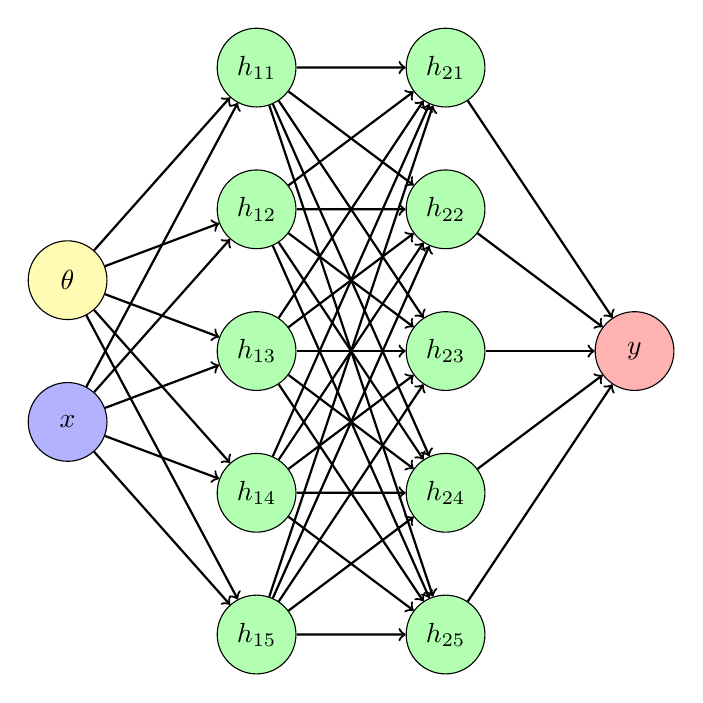
\begin{tikzpicture}[scale=1.2, every node/.style={draw, circle, minimum size=1cm}]
  % Input Layer
  \node[fill=yellow!30] (input1) at (0,0.75) {$\theta$};
  \node[fill=blue!30] (input2) at (0,-0.75) {$x$};

  % Hidden Layers
  \node[fill=green!30] (hidden11) at (2, 3.0) {$h_{11}$};
  \node[fill=green!30] (hidden12) at (2, 1.5) {$h_{12}$};
  \node[fill=green!30] (hidden13) at (2, 0.0) {$h_{13}$};
  \node[fill=green!30] (hidden14) at (2,-1.5) {$h_{14}$};
  \node[fill=green!30] (hidden15) at (2,-3.0) {$h_{15}$};

  \node[fill=green!30] (hidden21) at (4, 3.0) {$h_{21}$};
  \node[fill=green!30] (hidden22) at (4, 1.5) {$h_{22}$};
  \node[fill=green!30] (hidden23) at (4, 0.0) {$h_{23}$};
  \node[fill=green!30] (hidden24) at (4,-1.5) {$h_{24}$};
  \node[fill=green!30] (hidden25) at (4,-3.0) {$h_{25}$};

  % Output Layer
  \node[fill=red!30] (output) at (6, 0.0) {$y$};

  % Arrows
  \draw[->, thick] (input1) -- (hidden11);
  \draw[->, thick] (input1) -- (hidden12);
  \draw[->, thick] (input1) -- (hidden13);
  \draw[->, thick] (input1) -- (hidden14);
  \draw[->, thick] (input1) -- (hidden15);
  \draw[->, thick] (input2) -- (hidden11);
  \draw[->, thick] (input2) -- (hidden12);
  \draw[->, thick] (input2) -- (hidden13);
  \draw[->, thick] (input2) -- (hidden14);
  \draw[->, thick] (input2) -- (hidden15);

  \draw[->, thick] (hidden11) -- (hidden21);
  \draw[->, thick] (hidden11) -- (hidden22);
  \draw[->, thick] (hidden11) -- (hidden23);
  \draw[->, thick] (hidden11) -- (hidden24);
  \draw[->, thick] (hidden11) -- (hidden25);

  \draw[->, thick] (hidden12) -- (hidden21);
  \draw[->, thick] (hidden12) -- (hidden22);
  \draw[->, thick] (hidden12) -- (hidden23);
  \draw[->, thick] (hidden12) -- (hidden24);
  \draw[->, thick] (hidden12) -- (hidden25);

  \draw[->, thick] (hidden13) -- (hidden21);
  \draw[->, thick] (hidden13) -- (hidden22);
  \draw[->, thick] (hidden13) -- (hidden23);
  \draw[->, thick] (hidden13) -- (hidden24);
  \draw[->, thick] (hidden13) -- (hidden25);

  \draw[->, thick] (hidden14) -- (hidden21);
  \draw[->, thick] (hidden14) -- (hidden22);
  \draw[->, thick] (hidden14) -- (hidden23);
  \draw[->, thick] (hidden14) -- (hidden24);
  \draw[->, thick] (hidden14) -- (hidden25);

  \draw[->, thick] (hidden15) -- (hidden21);
  \draw[->, thick] (hidden15) -- (hidden22);
  \draw[->, thick] (hidden15) -- (hidden23);
  \draw[->, thick] (hidden15) -- (hidden24);
  \draw[->, thick] (hidden15) -- (hidden25);

  \draw[->, thick] (hidden21) -- (output);
  \draw[->, thick] (hidden22) -- (output);
  \draw[->, thick] (hidden23) -- (output);
  \draw[->, thick] (hidden24) -- (output);
  \draw[->, thick] (hidden25) -- (output);
\end{tikzpicture}
}
\caption{In the fitting step, the only trainable parameter is the yellow node representing $\theta$.}
\end{Pic}

\end{frame}

\subsubsection{SeaQuest MC Data Generation}

\begin{frame}
\frametitle{SeaQuest MC Data Generation}

\begin{List}{7.}{(1., 2.)}

    \item We generated the Monte Carlo (MC) data using the PYTHIA generator.

    \item The generated events were then passed through the E906 detector simulation (using GEANT4) to obtain the reconstructed detector information.

    \item We sample the values of $\lambda$, $\mu$ and $\nu$ uniformly  from the ranges of (0.5, 1.5), (−0.5, 0.5), and (−0.5, 0.5), respectively.\BeamerCite{NuSea:2006gvb}

\end{List}

\begin{Pic}{7.}{(8., 2.)}
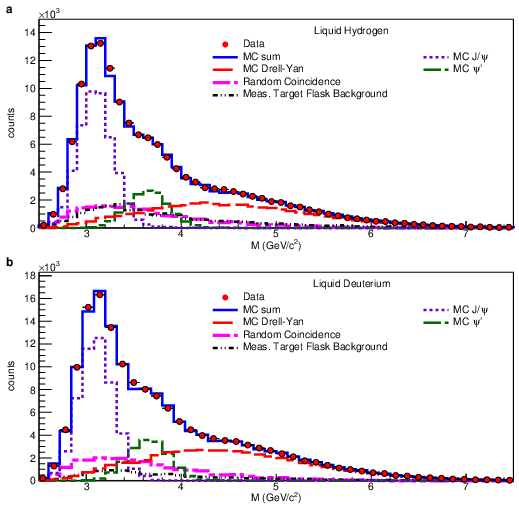
\includegraphics[width=6.cm]{imgs/mc2real.png}
    \caption{SeaQuest MC data is in good agreement with real data.\BeamerCite{SeaQuest:2021zxb}}
\end{Pic}

\end{frame}

\begin{frame}
\frametitle{Deep Neural Network Architecture}

\begin{List}{14.}{(1., 3.)}

    \item The neural network consists of five hidden linear layers, each containing 64 nodes. The ReLU function is used to activate the hidden layers, along with batch normalization layers. The final output is passed through a Sigmoid activation function.

    \item  During the training step, we use the following input features for the neural network: mass, $p_{T}$, $x_{F}$, $\phi$, $\cos\theta$, $\lambda$, $\mu$, and $\nu$.

    \item The neural network was trained for 200 epochs, employing early stopping with a patience of 20, to minimize the binary cross-entropy loss.

    \item During the fitting step, we freeze all the weights and biases of the trained neural network. Then, we employ the gradient descent algorithm to determine the optimal values of $\lambda$, $\mu$, and $\nu$ by minimizing the loss.

\end{List}

\end{frame}

\begin{frame}
\frametitle{Fitting Step}

\begin{Pic}{6.}{(1., 2.)}
    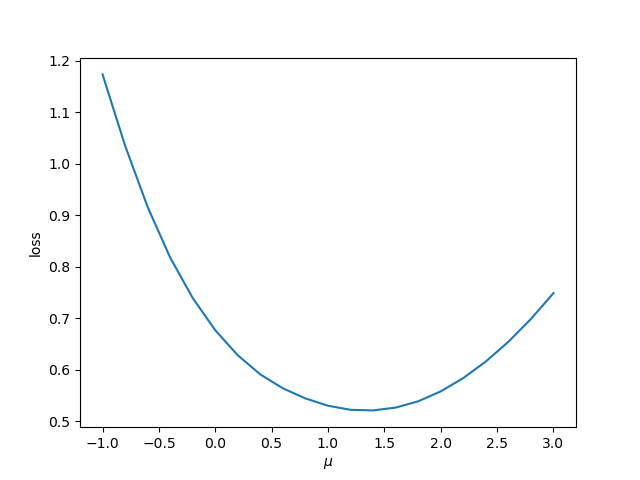
\includegraphics[width=6.0cm]{imgs/loss1D.png}
    \caption{In the fitting step, the loss reaches its minimum at the optimal value.}
\end{Pic}

\begin{Pic}{6.}{(8., 2.)}
    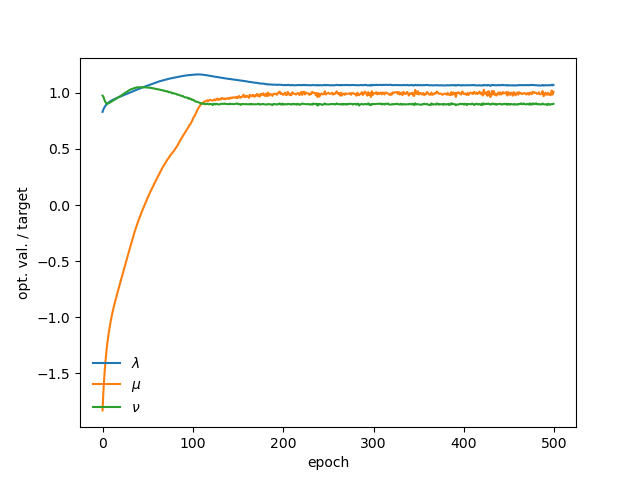
\includegraphics[width=6.0cm]{imgs/opt_fit_26.png}
    \caption{During the fitting step, all three parameters reach the optimal value.}
\end{Pic}

\end{frame}

\begin{frame}
\frametitle{Testing DNN approach}

\begin{textblock}{10.}(1., 2.)
\begin{center}
\begin{table}
\begin{tabular}{ |c| c| c| c| }
\hline
Combination & Coefficient & Injected & Fitted \\
\hline
1           & $\lambda$   & 0.84      & 0.876 $\pm$ 0.208 \\
            & $\mu$       & 0.26      & 0.234 $\pm$ 0.054 \\
            & $\nu$       & -0.34      & -0.299 $\pm$ 0.052 \\
\hline
2           & $\lambda$   & 1.33      & 1.134 $\pm$ 0.151 \\
            & $\mu$       & 0.17      & 0.146 $\pm$ 0.050 \\
            & $\nu$       & -0.34      & -0.281 $\pm$ 0.043 \\
\hline
3           & $\lambda$   & 1.12      & 1.242 $\pm$ 0.181 \\
            & $\mu$       & -0.27      & -0.211 $\pm$ 0.088 \\
            & $\nu$       & -0.24      & -0.236 $\pm$ 0.071 \\
\hline
% 4           & $\lambda$   & 0.62      & 0.888 $\pm$ 0.282 \\
%             & $\mu$       & -0.32      & -0.232 $\pm$ 0.091 \\
%             & $\nu$       & 0.18      & 0.147 $\pm$ 0.055 \\
% \hline

\end{tabular}
  \caption{Table showing the mean and standard deviation of fitted values of $\lambda$, $\mu$, and $\nu$ using the gradient descent algorithm with different model initialization.}
  \label{tabel:1}
\end{table}
\end{center}
\end{textblock}

\begin{List}{5.}{(11., 2.)}
  \item Independent events from training data $\rightarrow$ to reduce the biases

  \item 3 test sample $\rightarrow$ extract the injected parameters within a $\pm$1.5 standard deviation ($\sigma$) interval
\end{List}

\end{frame}

\subsection{Variational Autoencoders to Remove Combinatorial Background Events}

\begin{frame}
\frametitle{Combinatorial Background}

\begin{List}{14.}{(1., 2.)}

  \item Understanding the background from the experiment data is really important

  \item Full background simulations $\rightarrow$ computationally expensive

  \item Variational autoencoders;

  \begin{itemize}

    \item Generative model $\rightarrow$ can generate new events based on the trained events

    \item Computation is fast $\rightarrow$ use of GPUs

    \item Can use a higher-dimension inputs

    \item Control over the reconstruction error can be achieved using KL divergence

    \item Trained VAE $\rightarrow$ background subtracted events $\rightarrow$ un-binned method

  \end{itemize}

\end{List}

\end{frame}

\begin{frame}
\frametitle{Combinatorial Background}

\begin{Pic}{6.}{(8., 0.5)}
    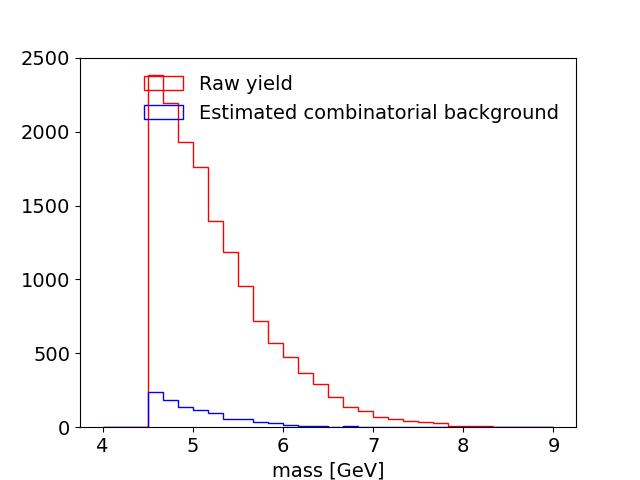
\includegraphics[width=6.0cm]{imgs/cmbg.png}
    \caption{Mix and un-mixed events.}
\end{Pic}

\begin{List}{7.}{(1.,2.)}

    \item We use an event-mixing method to estimate the combinatoric background from the SeaQuest data.\BeamerCite{SeaQuest:2023tcr}

    \item To remove the combinatorial background, we employ histogram subtraction $\rightarrow$ binned method, which does not scale well in higher dimensions

\end{List}

\begin{List}{14.}{(1., 11.)}

    \item Our goal is to utilize Variational Autoencoders (VAEs) for generating background-subtracted distributions.\BeamerCite{kingma2013auto}

    \item VAE generated distribution $\rightarrow$ fitting algorithm $\rightarrow$ $\lambda, \mu, \nu$

\end{List}

\end{frame}

\begin{frame}
\frametitle{VAEs}

\begin{Pic}{8.}{(1., 2.)}
    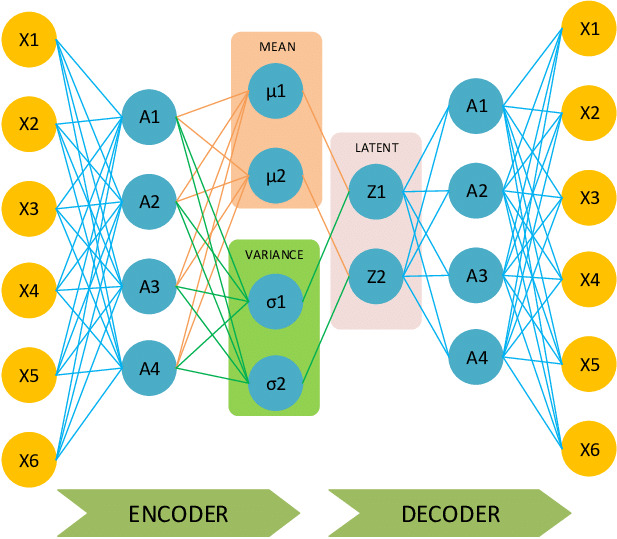
\includegraphics[width=8.0cm]{imgs/VAE.png}
    \caption{Example of VAE network.}
\end{Pic}

\begin{List}{6.}{(9., 2.)}

    \item Enforce the latent space to be Gaussian-like

    \item Generate noise vector in latent space $\rightarrow$ decode to generate sample

    \item Inputs: mass, $p_{T}$, $x_{F}$, $\phi$, $\cos\theta$

    \item Both the encoder and decoder have 3 hidden layers, each containing 64 nodes activated by the ReLU activation function.

    \item The latent dimension is 3.

\end{List}

\end{frame}

\begin{frame}
\frametitle{VAE Generated Events}

\begin{Pic}{5.}{(1., 1.)}
    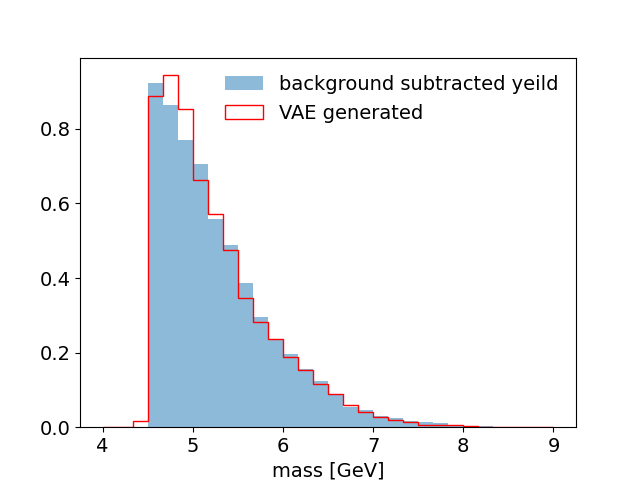
\includegraphics[width=5.0cm]{imgs/mass.png}
\end{Pic}

\begin{Pic}{5.}{(6., 1.)}
    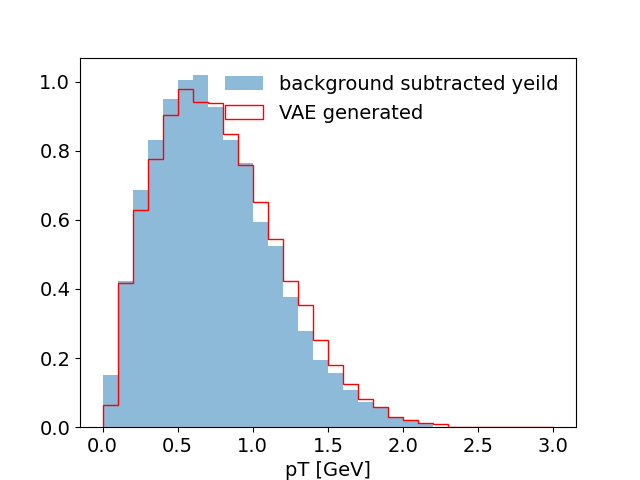
\includegraphics[width=5.0cm]{imgs/pT.png}
\end{Pic}

\begin{Pic}{5.}{(11., 1.)}
    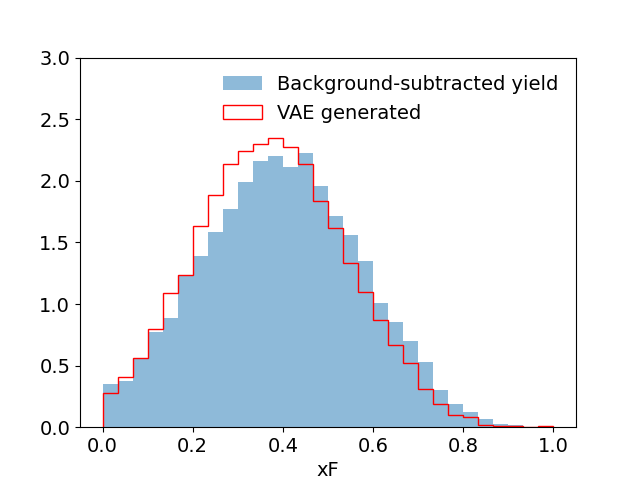
\includegraphics[width=5.0cm]{imgs/xF.png}
\end{Pic}

\begin{Pic}{5.}{(1., 8.)}
    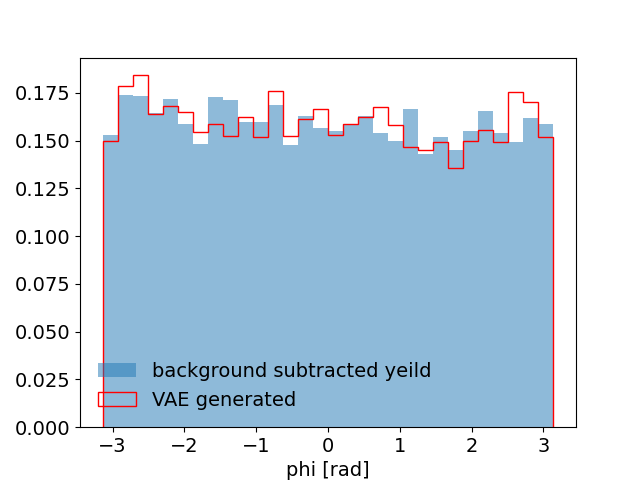
\includegraphics[width=5.0cm]{imgs/phi.png}
\end{Pic}

\begin{Pic}{5.}{(6., 8.)}
    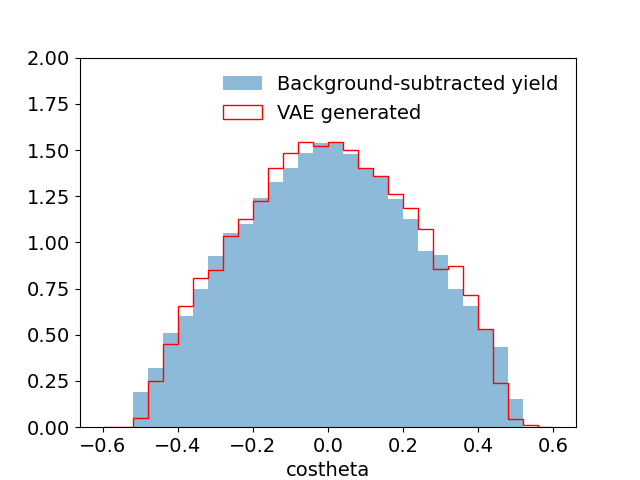
\includegraphics[width=5.0cm]{imgs/costh.png}
\end{Pic}

\begin{textblock}{5.0}(10.5, 10.)

Early result $\rightarrow$ enhance the prediction accuracy using diffusion models/ conditional VAEs.

\end{textblock}

\end{frame}

\begin{frame}
\frametitle{Future Trajectory}

\begin{List}{14.}{(1., 2.)}

  \item Systematic study of the fitting algorithm to better understand the phase space variables.

  \item Increase the precision of the fitting algorithm using VAE/GAN.\BeamerCite{Diefenbacher:2020rna}

  \item Increase the accuracy of the prediction for background-subtracted events with Diffusion/CVAE models.

\end{List}

\end{frame}

\section{Summary}

\begin{frame}
\frametitle{Summary}

\begin{List}{14.0}{(1., 2.)}

    \item Spin of the proton $\rightarrow$ intrinsic property $\rightarrow$ explain the structure of the proton

    \item BM function $\rightarrow$ transverse-polarization asymmetry of quarks within an unpolarized hadron

    \item Neural networks $\rightarrow$ multi-dimensional likelihood functions $\rightarrow$ likelihood ratio test to extract the optimal parameters for the Drell-Yan angular distribution.

    \item VAEs $\rightarrow$ generate distributions with background removed.

    \item Our plan is to use this high-dimensional fitting algorithm with VAE generated events to extract the Drell-Yan angular coefficients from the E906/SeaQuest data with higher accuracy.

    \item Acknowledgement: This work was funded by the DOE office of Science, Medium-Energy Nuclear Physics Program.

\end{List}
\end{frame}

\end{document}
